\section{Commercial Fusion}
\begin{frame}{Commercial Fusion}
    \begin{itemize}
        \item I will talk about General Fusion's fusion reactor.
        \item I think it is useful to include a list of companies working on fusion energy.
              \url{https://en.wikipedia.org/wiki/Commercial_fusion}
        \item General Fusion uses a structure called Magnetized Target Fusion.
    \end{itemize}
\end{frame}

\begin{frame}{General Fusion - Magnetic Target Fusion}
    \begin{figure}
        \centering
        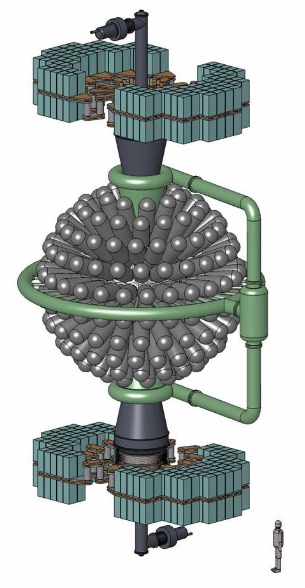
\includegraphics[width=0.3\textwidth]{figures/gf-structure.png}
        \caption{\cite{DelageM.2012PtaM} General Fusion's Acoustic Magnetized Target Fusion Reactor Concept.}
    \end{figure}
\end{frame}

\begin{frame}{General Fusion - Plasma in Field-Reverse Configuration}
    \begin{itemize}
        \item Plasma injectors inject spheromaks with opposite helicity into the center.
        \item Spheromaks meet and form a plasma that is in field reverse configuration (FRC).
        \item Plama in FRC is stable, so no need for the coils. \cite{LabergeMichel2009ERfa}
    \end{itemize}

    \begin{figure}
        \centering
        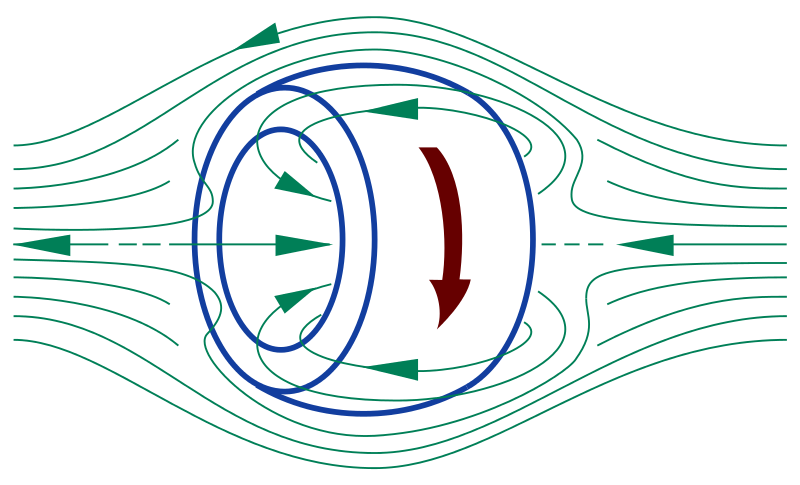
\includegraphics[width=0.3\textwidth]{figures/frc.png}
        \caption{Field-reversed configuration: a toroidal electric current is induced inside a cylindrical plasma, making a poloidal magnetic field, reversed in respect to the direction of an externally applied magnetic field. The resultant high-beta axisymmetric compact toroid is self-confined. Taken from \url{https://commons.wikimedia.org/wiki/File:Field-Reversed_Configuration.svg}}
    \end{figure}
\end{frame}

\begin{frame}{General Fusion - Liquid Pb-Li as Blanket}
    In order to absorb the neutrons emitted from the fusion reaction, a liquid metal, Pb-Li, is used as the blanket. Moreover, the Li element can help to breed the tritium through the reaction, $^7Li+n \to ^4He + ^3H + n$, for further fusion reaction. \cite{LabergeMichel2009ERfa}
    \begin{itemize}
        \item Pb-Li liner is spun up in the device to wrap the plasma.
        \item Steam piston compresses all the things to create fusion.
        \item Liquid metal liner is extracted for heat exchange purpose.
    \end{itemize}

    \begin{figure}
        \centering
        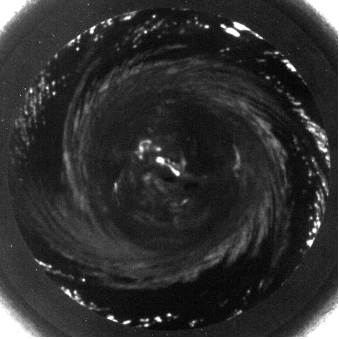
\includegraphics[width=0.3\textwidth]{figures/liquid-pb.png}
        \caption{Image of Liquid Pb.}
    \end{figure}
\end{frame}